% -----------------------------------------------------------------------------
% main_v5.tex - fifth draft of the Tethys data paper.
% Revisions in this version address co-author comments from v4 and verify
% that every \cite{} resolves to a real bibliography entry.
% -----------------------------------------------------------------------------

\documentclass[fleqn,10pt]{wlscirep}
%\usepackage[utf8]{inputenc}
\usepackage[T1]{fontenc}
\usepackage{textcomp}
\usepackage{lineno}
\usepackage{booktabs}

\usepackage{tikz}
\usetikzlibrary{positioning, arrows.meta, fit, backgrounds, shapes.geometric}

\usepackage{graphicx}
\graphicspath{{figures/}}

%\usepackage{biblatex}
%\addbibresource{bib/Tethys.bib} 

\linenumbers

% \title{High-resolution 21st-century monthly water demands for the contiguous United States}
\title{High-resolution monthly sectoral water demands for the U.S. over 1980-2100} % across diverse futures

\author[1*]{Cameron Bracken}
\author[2*]{Hassan Niazi}
\author[1]{Travis Thurber}
\author[2]{Isaac Thompson}
\author[1]{Kazi Tamaddun}
\author[3]{Hisham Eldardiry}
\author[1]{Kendall Mongird}
\author[1,3]{Nathalie Voisin}
\author[1]{Ning Sun}
\author[1]{Jennie Rice}

\affil[1]{Pacific Northwest National Laboratory, Richland, WA, USA}
\affil[2]{Joint Global Change Research Institute, Pacific Northwest National Laboratory, College Park, MD, USA}
\affil[3]{University of Washington, Seattle, WA, USA}

\affil[*]{corresponding author(s): Cameron Bracken (cameron.bracken@pnnl.gov), Hassan Niazi (hassan.niazi@pnnl.gov)}

\begin{abstract}
U.S. water demand varies sharply by sector and region as land use, population, weather patterns, and economic activity co-evolve. High-resolution water demand data are required to capture these dynamics and to support integrated energy-water-land modeling and local-to-regional water scarcity assessments. We present a gridded (1/8$^{\circ}$), monthly, multi-sector water demand dataset for the contiguous United States (CONUS) covering 1980--2100 across one historical period and eight future scenarios spanning a wide but plausible range of atmospheric conditions, emissions constraints, and economic, technological, and population growth assumptions. The dataset covers six demand sectors --- irrigation, thermoelectric, municipal (public-supply and domestic), livestock, manufacturing, and mining --- aggregated from 25 underlying subsectors, separately for withdrawals and consumption, and includes per-cell groundwater and surface-water source attributions. The historical record is validated against the United States Geological Survey (USGS) 2010--2020 water-use reanalysis for the three largest sectors at the Hydrologic Unit Code 6 (HUC6) scale, with Pearson correlations from 0.73 to 0.95. The dataset advances prior global products through state-resolved sectoral demands, future power-plant siting projections, scenario-consistent population and land-use forcing, and a spatial-resolution refinement from 1/2$^{\circ}$ to 1/8$^{\circ}$.
\end{abstract}
\begin{document}

\flushbottom
\maketitle
% Click the title above to edit the author information and abstract

\thispagestyle{empty}

% -----------------------------------------------------------------------------
\begin{figure}[!ht]
\centering

\includegraphics[width=\linewidth]{usage1-dominant-sector-tethys-grid.png}
\caption{Dominant water-use sector at each 1/8$^{\circ}$ cell across CONUS, by annual-average consumption in the historical Tethys output (1980--2019). Spatial patterns reflect the multi-sector and heterogeneous nature of U.S. water demand, such as irrigation across the Great Plains, Mountain West, and Central Valley; thermoelectric concentrated near major generation centers in the Southeast and along the major navigable rivers; domestic demand surrounding metropolitan areas; livestock, manufacturing, and mining adding regional structure. These patterns underscore the need for high-resolution, multi-sector datasets that prior global products could not capture.}
\label{fig:dominant-sector}
\end{figure}

\section*{Background \& Summary}

Humans depend on water for irrigation, thermoelectric cooling, municipal, industrial, and livestock purposes. The relative contribution of these sectors varies sharply across regions and over time. Global water demand is projected to rise through the 21st century under combined socioeconomic pressures and evolving weather patterns\cite{WWDR2019, Niazi2024PeakWater, Awais2024Preprint}. Demand-side drivers, not supply-side limits, dominate most projected shifts in water scarcity\cite{Graham_2020, Awais2024Preprint, Kyle2023Sustainability}. Even where regional supply appears ample, scarcity can manifest locally when demand and availability are mismatched in space or time\cite{HADJIMICHAEL23}. Modeling water scarcity under complex and dynamic future conditions requires demands resolved at the spatial and temporal scales relevant to management decisions.

High-resolution, multi-sector water-demand projections remain scarce, constraining integrated modeling of energy-water-land systems and local-to-regional water scarcity. Reconstructed historical datasets, such as Huang et al. (2018)\cite{Huang2018}, provide gridded benchmarks for past decades but do not extend to future scenarios. Projecting water demand into the future requires an integrated assessment model that link global energy, land, and water systems, yet their outputs typically lack the spatial detail required for river routing or local management modeling\cite{Wada_2017, van_Vliet_2021}. While aggregate U.S. water demands at coarse resolutions are generally consistent in the literature \cite{Zhao_gcamusa_water, naseri2025united, Stets2025USGS}, translating them to finer scales requires spatial and temporal downscaling\cite{hess-17-4555-2013, van_Vliet_2021, Jones_2024}. The fidelity of downscaling depends strongly on the choice of proxy variables and the consistency of driving scenarios. Khan et al. (2023)\cite{Khan2023} produced the first global Tethys-downscaled multi-sector water demand product at 1/2$^{\circ}$ monthly resolution; resolving CONUS-scale management decisions and understanding local-scale impacts, however, requires finer spatial resolution and internally consistent scenario forcings of weather, land-use, and population.

We present such a dataset with multisector, multi-scenario coverage, refined to 1/8$^{\circ}$ monthly resolution across CONUS. The published record contains gridded monthly water withdrawals and consumption for six sectors --- irrigation, thermoelectric, municipal (public-supply and domestic), livestock, manufacturing, and mining --- aggregating 25 underlying GCAM-USA subsectors (11 crop and land-use types, 7 thermoelectric generation types, 5 livestock species, plus municipal, manufacturing, and mining). Dataset extent covers CONUS for the historical period (1980--2019) and eight future scenarios (2020--2100) sampling future atmospheric and socioeconomic conditions. For each scenario, the dataset also provides per-cell groundwater-to-surface-water source fractions. The downscaling chain improves on the prior Tethys global product in six specific ways: (1) U.S. state-level water demands from the Global Change Analysis Model with subnational detail for the U.S. (GCAM-USA \cite{Zhao_gcamusa_water,Zhao2024,Calvin2019GCAM,Binsted_2022}), (2) explicit Capacity Expansion Regional Feasibility (CERF) \cite{Vernon2021} power-plant siting consistent with GCAM-USA capacity-expansion projections through 2100, (3) SSP scenario-consistent population proxies, (4) seasonally dependent temporal downscaling of irrigation using growing-season-index (GSI) deficits, (5) groundwater/surface-water source-share adjustments anchored to USGS observations, and (6) a resolution refinement from 1/2$^{\circ}$ to 1/8$^{\circ}$ (see Section~\ref{sec:improvements}, ``Improvements over previous data sets'', for details).

A representative result is shown in Figure~\ref{fig:dominant-sector}, presenting dominant demand sector at each 1/8$^{\circ}$ cell across CONUS in the historical record (1980-2020). The result demonstrates the dynamic multi-sector nature of water demands in CONUS, which motivates the rest of the paper. The dataset is expected to support hydrologic, energy-water-land, and integrated multisector dynamics modeling, and research on U.S.\ bulk-power-system resilience, water scarcity, and groundwater/surface water interactions, by providing a consistent foundation across scenarios that enables inter-model comparisons. 


\begin{table}[!ht]
\centering
\small
\begin{tabular}{lllll}
\toprule
\textbf{Dataset} & \textbf{Spatial res.} & \textbf{Temporal res.} & \textbf{Scenarios} & \textbf{Sectors} \\
\midrule
Huang et al.\cite{Huang2018}                   & 0.5$^{\circ}$ global & monthly & historical (1971--2010) & 6 sectors \\
Khan et al.\cite{Khan2023}    & 0.5$^{\circ}$ global & monthly & historical + SSP/RCP futures & 6 sectors \\
Medalie et al.\cite{Stets2025USGS}             & HUC12 CONUS & monthly & historical (2010--2020) & 3 sectors \\
Naseri \& Marston\cite{naseri2025united}       & facility/user-level, & annual & historical & multi-sector  \\
                                               & 42 U.S. states & (state-dependent) &  &   \\
van Vliet et al.\cite{van_Vliet_2021}          & country/basin & annual & historical + SSP & 6 sectors \\
Wada et al.\cite{Wada_2017}                    & 0.5$^{\circ}$ global & monthly & historical + projections & 4 sectors \\
\textbf{This work}                             & \textbf{0.125$^{\circ}$ CONUS} & \textbf{monthly} & \textbf{hist.\ + 2 RCPs $\times$ 2 GCMs $\times$ 2 SSPs} & \textbf{6 sectors} \\
                                               &                                &                  & \textbf{(8 future scenarios)}                                & \textbf{(25 subsectors)} \\
                                               
                                               &                                &               &                  & \textbf{+ gw/sw source split} \\
\bottomrule
\end{tabular}
\caption{Gridded multi-sector water-demand datasets that overlap in scope with the dataset presented here. The current dataset increases spatial resolution by a factor of four (16$\times$ the number of grid cells) over its immediate Tethys predecessor\cite{Khan2023}, adds per-cell groundwater-to-surface-water source attribution, and uses internally consistent scenarios of population, land-use, and climate forcing. The six sectors aggregate 25 underlying GCAM-USA subsectors: 11 crop and land-use types (irrigation), 7 thermoelectric generation types (electricity), 5 livestock species, plus municipal, manufacturing, and mining.}
\label{tab:prior-datasets}
\end{table}

% -----------------------------------------------------------------------------
\section*{Methods and Data}
We produce the dataset by applying Tethys\cite{niazi_2026_20552731} (\href{https://github.com/JGCRI/tethys}{github.com/JGCRI/tethys}), a mass-conserving spatiotemporal downscaling framework, to GCAM-USA outputs together with sector-specific spatial proxies and intra-annual temporal downscaling weights derived from meteorology. The result is a 1/8$^{\circ}$ monthly water-demand record for 6 sectors and 25 GCAM-USA subsectors, for one historical period (1980--2019) and eight future scenarios (2020--2100). Table~\ref{tab:prior-datasets} compares this dataset with closely related published records, highlighting advances in spatial resolution, scenario breadth, and groundwater/surface-water attribution. The Tethys downscaling chain (Figure~\ref{fig:schematic}) converts state- and basin-scale water-demand projections from GCAM-USA\cite{Zhao_gcamusa_water,Zhao2024,Calvin2019GCAM,Binsted_2022} into 1/8$^{\circ}$ monthly gridded fields by applying sector-specific spatial proxies --- land use (Demeter\cite{Vernon-2018}), power-plant siting (CERF\cite{Zhao2024,Mongird2025CERF}), population (Jones \& O'Neill SSPs\cite{Jones_2016}), and livestock (GLW~3\cite{Gilbert2018}) --- and distributing the annual values into months using meteorological indicators derived from the TGW\cite{Jones2023TGW} dataset (deficit, growing-season index, heating- and cooling-degree days). A final post-processing step assigns each cell's groundwater-to-surface-water supply share based on basin-level source splits. The downscaling process is repeated for each of the eight scenarios.

The remainder of this section is organized in two parts. The first part describes the exogenous scenarios and inputs to Tethys: GCAM-USA state- and basin-scale water demands, the TGW meteorological forcing, the Demeter land-use projections, and the CERF power-plant projections. The second part describes the Tethys mechanics: the spatial-downscaling step (Eq.~\ref{eq:spatial}) with sector-specific proxies, the temporal-downscaling step with sector-specific monthly weights, and the groundwater-to-surface-water source-share post-processing (Eq.~\ref{eq:source-shares}). The closing subsection documents the modular one-way coupling design.

\begin{figure}[!ht]
\centering
% Workflow figure is built natively in TikZ and compiled separately as a
% standalone PDF. Source: flow-chart.tex; rebuild with `pdflatex flow-chart.tex`.
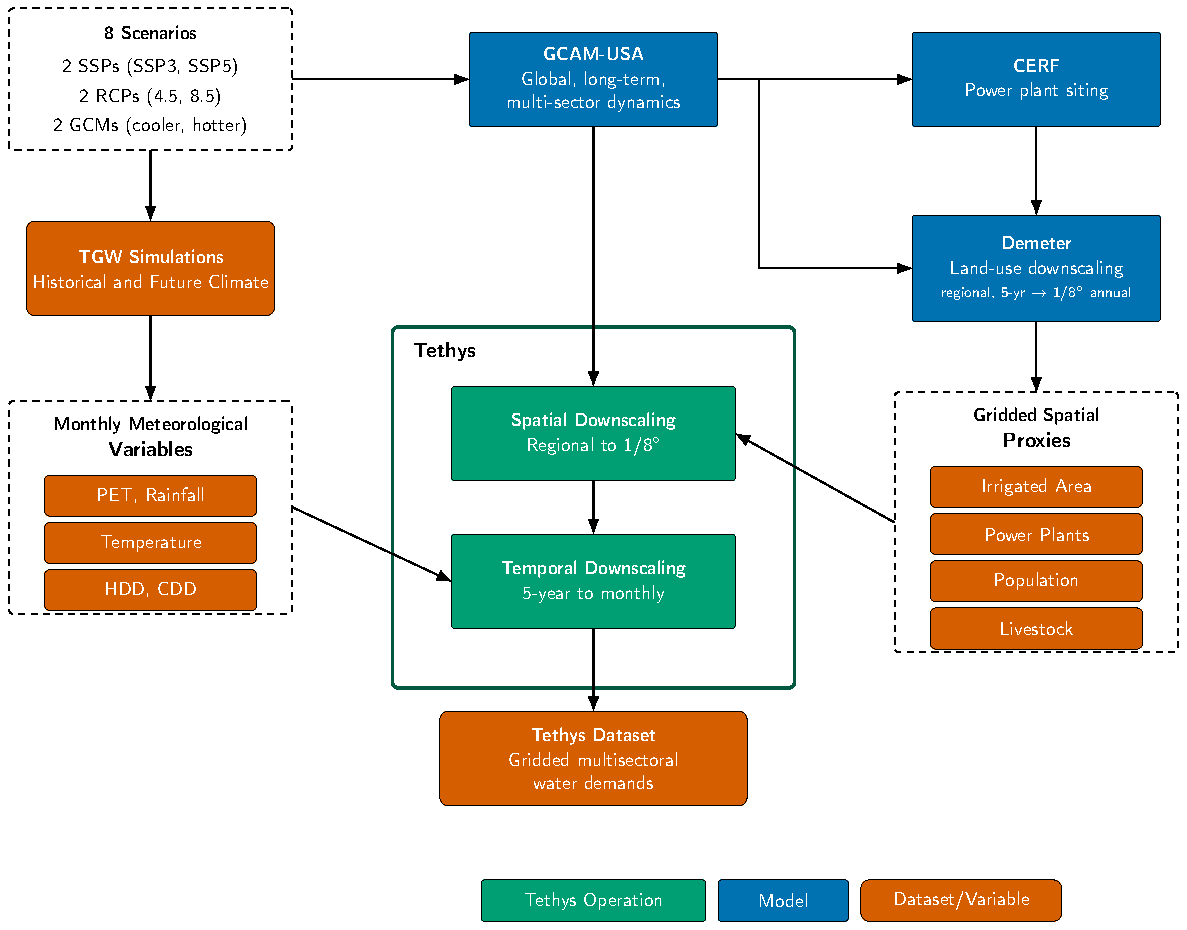
\includegraphics[width=0.9\textwidth]{figures/flow-chart.pdf}
\caption{Workflow for producing the Tethys CONUS multi-sector water-demand dataset for eight scenarios (Table~\ref{tab:scenarios}).  The eight scenarios combine two RCP forcing levels (4.5 and 8.5 W/m²), two GCM temperature-sensitivity groups (hotter and cooler), and two socioeconomic pathways (SSP3 and SSP5) FOr each scenario, Tethys (green boxes) carries out the two downscaling operations: spatial downscaling from regional aggregate demands to the 1/8$^{\circ}$ CONUS grid, and temporal downscaling of 5-year GCAM-USA outputs to monthly resolution. Spatial downscaling uses gridded proxies derived from Demeter\cite{Vernon-2018} (land use), CERF\cite{Zhao2024,Mongird2025CERF} (projected power-plant siting), Jones and O'Neill\cite{Jones_2016} (SSP-compliant population), and GLW~3\cite{Gilbert2018} (livestock). Temporal downscaling uses monthly meteorological variables derived from TGW\cite{Jones2023TGW}, including potential evapotranspiration (PET), precipitation, mean temperature, heating degree days (HDD), cooling degree days (CDD), and growing-season index (GSI).} 
\label{fig:schematic}
\end{figure}

\subsection*{GCAM-USA state/basin-Level Water demand}

Region-scale water-demand inputs come from the Global Change Analysis Model (GCAM-USA version)\cite{Zhao_gcamusa_water,Zhao2024,Calvin2019GCAM,Binsted_2022}. GCAM is a market-equilibrium integrated assessment model that allocates supply and demand across coupled energy, water, land, and economic sectors under scenario-specific assumptions on population, productivity, technology, and policy. GCAM-USA resolves U.S.\ electricity generation, manufacturing, and municipal demands at the state level and crop-level irrigation demands at state/basin intersections, at 5-year intervals. 5-year demands are linearly interpolated to annual demands before temporal downscaling is applied. Each of the eight runs corresponds to one scenario; we refer readers to Mongird et al.\cite{Mongird2025CERF}, Zhao et al.\cite{Zhao_gcamusa_water}, and Binsted et al.\cite{Binsted_2022} for the full energy-water-land coupling description of GCAM-USA and limit ourselves here to how the GCAM-USA outputs feed the Tethys workflow shown in Figure~\ref{fig:schematic}.

The dataset's historical period spans 1980--2019 and future scenarios span 2020--2100 across 8 scenarios\cite{Zhao_gcamusa_water,Zhao2024,Mongird2025CERF}. The future scenarios include three dimensions: emissions constraints (rcp45 = moderate constraints and moderately hotter and drier conditions, rcp85 = no constraints and severely hotter and drier conditions), GCM-temperature sensitivity over CONUS (cooler vs.\ hotter CMIP6 model groups), and Shared Socioeconomic Pathway (SSP3 = low population/economic growth, SSP5 = high growth). We use the acronym ``rcp'' for brevity in scenario names, although the underlying perturbed-thermodynamics simulations are derived from CMIP6, not CMIP5\cite{Mongird2025CERF}. The eight scenario directory names in the dataset (e.g., \texttt{rcp45cooler\_ssp3}) appear in Table~\ref{tab:scenarios} and the inter-scenario behavior of CONUS demand is shown in Figure~\ref{fig:scenarios}.

\subsection*{Meteorological forcing (TGW)}

Historical and projected meteorological data are from perturbed thermodynamics experiments \cite{Jones2023TGW} (\href{https://tgw-data.msdlive.org/}{tgw-data.msdlive.org}) which provides hourly atmospheric variables at 1/8$^{\circ}$ over CONUS, dynamically downscaled with WRF from a 30-km ERA5 historical baseline (1980--2019) and from CMIP6-derived monthly thermodynamic perturbations (2020--2100). The TGW approach replays historical weather sequences with added thermodynamic signals, retaining the synoptic structure of observed weather while shifting its mean state to match each future scenario. For each TGW scenario we compute daily potential evapotranspiration (PET), precipitation ($P$), mean temperature, heating degree days (HDD), cooling degree days (CDD), and a growing-season index (GSI). These are aggregated to monthly totals or means and reprojected to the Tethys 1/8$^{\circ}$ CONUS grid.

The monthly water deficit used in irrigation temporal downscaling is $\Delta_m = \max\!\big(\text{PET}_m - P_m,\, 0\big)$. The monthly GSI is derived from a simplified version of Jolly et al.\cite{Jolly_2005}, retaining the daily minimum-temperature ($iT_{\min}$) and daylength photoperiod indicators ($iPhoto$) but omitting the vapour-pressure-deficit term. For each day $d$,
\begin{equation}
iT_{\min,d}(T_{\min,d}) = \min\!\left(\max\!\left(\frac{T_{\min,d}+2}{7},\,0\right),\,1\right), \qquad
iPhoto_d(L_d) = \min\!\left(\max\!\left(L_d - 10,\,0\right),\,1\right),
\label{eq:gsi-components}
\end{equation}
where $T_{\min,d}$ is the daily minimum air temperature (\textdegree C) and $L_d$ is the daylength (hours). Monthly GSI is the daily-mean product over the month $m$,
\begin{equation}
GSI_m = \big\langle iT_{\min,d} \cdot iPhoto_d \big\rangle_{d \in m}.
\label{eq:gsi-monthly}
\end{equation}
Preprocessing code is archived in the integration meta-repository (see Code availability).

\subsection*{Downscaled Land-use projections (Demeter)}

Spatially explicit, scenario-consistent annual per-crop irrigated-area maps at 1/8$^{\circ}$ come from Demeter\cite{Vernon-2018}, a land-use spatial disaggregation model that reconciles a high-resolution land-use baseline with GCAM-USA's regional LULCC projections using transition-priority rules that distinguish intensification (increase of a land type within a cell) from extensification (spread from an adjacent cell). For irrigation, Demeter outputs cover the 13 crop classes that GCAM-USA reports (Corn, Wheat, Rice, RootTuber, OilCrop, SugarCrop, OtherGrain, FiberCrop, FodderGrass, FodderHerb, biomass, MiscCrop, PalmFruit). The per-crop irrigated-area fields serve as the spatial proxy for irrigation in the Tethys spatial-downscaling step (see following section for details).

\subsection*{Power-plant siting projections (CERF)\label{sec:cerf}}

The Capacity Expansion Regional Feasibility (CERF) model\cite{Vernon2021,Mongird2025CERF} sites future thermoelectric capacity at $\approx$1-km resolution based on siting feasibility (exclusion layers, transmission proximity, cooling-water access) and locational economics, conditional on the GCAM-USA state-level capacity trajectory for each scenario. The plants represent thermoelectric generation (coal, natural gas, oil, nuclear, biomass, geothermal, concentrated solar thermal), excluding hydropower. CERF-sited plants are aggregated to 1/8$^{\circ}$ grid cells, and the cell-level installed capacity (MW) serves as the spatial proxy for thermoelectric demand. For the historical period we substitute the 2015 plant inventory from the Global Power Plant Database v1.3 (GPPD)\cite{globalpowerplantdb} in place of CERF projections; both feed the same spatial-downscaling step at the cell.

\subsection*{Spatial downscaling}

Using the sector-specific proxies described above, Tethys distributes regional demands to the 1/8$^{\circ}$ grid. The spatial downscaling in Tethys operates under the assumption that the location of demand within a region follows a gridded proxy appropriate to the sector. For any sector with total demand $D_{\mathrm{region}}$ and proxy field $P_{\mathrm{cell}}$,
\begin{equation}
D_{\mathrm{cell}} = D_{\mathrm{region}} \times \frac{P_{\mathrm{cell}}}{\sum_{c \in \mathrm{region}} P_{c}}.
\label{eq:spatial}
\end{equation}
For irrigation, the proxy is per-crop irrigated area from Demeter (described above). For thermoelectric, the proxy is CERF-sited installed capacity (described in ``Power-plant siting projections'' above). For municipal demand, we use the scenario-consistent gridded population at 10-year intervals from Jones and O'Neill\cite{Jones_2016}, linearly interpolating between bracketing decadal maps, with state-level GCAM-USA municipal demand allocated to cells in proportion to projected population. For livestock, the proxy is the GLW~3 gridded head-count map\cite{Gilbert2018} at 1/12$^{\circ}$ for reference year 2010, re-gridded to 1/8$^{\circ}$ using weighted area-overlap allocation and held fixed across all years and scenarios; livestock is \textasciitilde2\% of CONUS demand, so the static-distribution assumption has limited overall impact (see Limitations). The mapping from GCAM livestock sectors to GLW animals follows Table~\ref{tab:livestock}. For manufacturing and mining, we use population as the spatial proxy, following prior Tethys work\cite{Khan2023}.

\begin{table}[!ht]
\centering
\begin{tabular}{ll}
\toprule
\textbf{GCAM livestock sector} & \textbf{GLW proxy animal(s)} \\
\midrule
Beef      & Buffalo + Cattle \\
Dairy     & Buffalo + Cattle \\
Pork      & Pig \\
Poultry   & Chicken + Duck \\
SheepGoat & Sheep + Goat \\
\bottomrule
\end{tabular}
\caption{Mapping from GCAM livestock sectors to animal species in the GLW~3 dataset.}
\label{tab:livestock}
\end{table}

\subsection*{Temporal downscaling}

For temporal downscaling. we linearly interpolate spatially-downscaled outputs to annual resolution and then distribute the annual demand at each cell into 12 monthly values using sector-specific formulas. For livestock, manufacturing, and mining we hold monthly demand uniform at $1/12$ of the annual total; irrigation, electricity, and municipal follow formulations described next.

\subsubsection*{Irrigation}

For each cell and year, we compute a monthly weight field from the growing-season index $GSI_m$ (Eq.~\ref{eq:gsi-monthly}), the monthly deficit $\Delta_m$, and month length $N_m$ (in days):
\begin{equation}
\tilde{w}_m = \frac{\Delta_m \, GSI_m}{N_m}\quad, \qquad w_m = \frac{\tilde{w}_m}{\sum_{k=1}^{12}\tilde{w}_k},
\label{eq:irr-weights}
\end{equation}
so $\sum_m w_m = 1$ and monthly irrigation demand is $D_{Irrigation,m} = w_m \, D_{Irrigation,\mathrm{year}}$. Equation~(\ref{eq:irr-weights}) combines the deficit and growing season approaches of Moore et al.\cite{Moore_2015} and Roy et al.\cite{Roy_2005}. Using this approach, water demand concentrates in months that are simultaneously water-limited ($\Delta_m > 0$) and vegetatively active ($GSI_m > 0$). The weights are computed per cell and differ across years.

\subsubsection*{Electricity}

We distribute monthly thermoelectric cooling water demand by splitting annual use into heating, cooling, and other shares, each weighted by an HDD/CDD-driven monthly profile. Region-level shares of annual electricity consumption for heating $p_{\mathrm{heat}}$, cooling $p_{\mathrm{cool}}$, and other $p_{\mathrm{other}}$ come from GCAM-USA. At each cell we define annual sums $H_y = \sum_m \text{HDD}_m$ and $C_y = \sum_m \text{CDD}_m$ and monthly distribution fields $\hat{h}_m$ and $\hat{c}_m$ with
\begin{equation}
(\hat{h}_m,\,\hat{c}_m) =
\begin{cases}
\big(\text{HDD}_m / H_y,\ \text{CDD}_m / C_y\big)      & H_y \ge 650 \text{ and } C_y \ge 450 \\[2pt]
\big(\text{HDD}_m / H_y,\ \text{HDD}_m / H_y\big)      & H_y \ge 650 \text{ and } C_y < 450 \\[2pt]
\big(\text{CDD}_m / C_y,\ \text{CDD}_m / C_y\big)      & H_y < 650 \text{ and } C_y \ge 450 \\[2pt]
(\hat{o},\ \hat{o})                                          & H_y < 650 \text{ and } C_y < 450,
\end{cases}
\label{eq:elec-cases}
\end{equation}
with $\hat{o} = 1/12$. 
The first case applies to cells with both a meaningful heating season (annual HDD $\ge 650$) and a meaningful cooling season (annual CDD $\ge 450$). The second and third cases collapse onto whichever signal is non-trivial, preventing division by near-zero annual sums in climates dominated by one extreme. The fourth case reverts to a uniform distribution where neither threshold is exceeded. The threshold convention follows Huang et al.\cite{Huang2018}. Once $\hat{h}_m$ and $\hat{c}_m$ are computed, monthly demand is then downscaled from annual ($D_{Electricity,m}$) demand ($D_{Electricity,\mathrm{year}}$)
\begin{equation}
D_{Electricity,m} = D_{Electricity,\mathrm{year}} \times \big(p_{\mathrm{heat}}\,\hat{h}_m + p_{\mathrm{cool}}\,\hat{c}_m + p_{\mathrm{other}}\,\hat{o}\big).
\label{eq:elec-demand}
\end{equation}


\subsubsection*{Municipal}

For the municipal sector (covering domestic/public-supply), we use the temperature-anomaly formula of Wada et al.\cite{Wada2011}:
\begin{equation}
D_{Municipal,m} = \frac{D_{Municipal,\mathrm{year}}}{12} \times \left(\frac{T_m - \bar{T}}{T_{\max} - T_{\min}}\,R + 1\right),
\label{eq:dom-monthly}
\end{equation}
where $T_m$ is the monthly mean temperature at the cell, $\bar{T}$ is the annual mean temperature, $T_{\max}$ and $T_{\min}$ are the annual extremes, and $R$ is a region-scale amplitude coefficient drawn from a static regional map; higher $R$ implies stronger seasonal amplification. We clip negative values to zero so that $D_{Municipal,m} \ge 0$ in every cell. Note that USGS refers to the municipal sector as Public Supply, which can encompass Domestic and Industrial water use that is supplied by publicly owned water rights.

\subsection*{Groundwater vs.\ surface water source-share post-processing}

GCAM-USA solves for the share of each basin's withdrawals met from surface versus groundwater supply using cost-based allocation of supply sources to competing sectoral demands. Mapping that basin-scale split onto the 1/8$^{\circ}$ grid requires two steps. First, we apply the basin-level share uniformly to all water-use sectors in the basin, except that thermoelectric demand is assumed to use surface water only, and the remaining sectoral shares are renormalized accordingly. Second, we anchor the historical spatial pattern of the groundwater-to-surface split to USGS data by rescaling each cell's GCAM share against its 2015 value while preserving the spatial pattern of a static USGS baseline derived from the 2009-2020 mean groundwater-to-surface share distribution\cite{Stets2025USGS}. Let $s^{\mathrm{GCAM}}_{c,y}$ denote the GCAM-derived renewable share at cell $c$ in year $y$, and $s^{\mathrm{USGS}}_c$ the static USGS-derived baseline share at cell $c$. For the subset of cells $\mathcal{M}$ for which both $s^{\mathrm{GCAM}}_{c,\,2015}>0$ and $s^{\mathrm{USGS}}_c$ are available, the adjusted share is
\begin{equation}
s^{\mathrm{adj}}_{c,y} =
\begin{cases}
\displaystyle \min\!\left(1,\; s^{\mathrm{USGS}}_c \times \frac{s^{\mathrm{GCAM}}_{c,y}}{s^{\mathrm{GCAM}}_{c,\,2015}}\right) & c \in \mathcal{M} \\[10pt]
s^{\mathrm{GCAM}}_{c,y}                                                                                        & c \notin \mathcal{M}.
\end{cases}
\label{eq:source-shares}
\end{equation}
The expression $\min(\cdot,1)$, limits shares to a maximum value of 1, preventing unrealistically large values when the 2015 GCAM baseline is small. In groundwater-dominated regions, the limit can suppress increases in projected trajectories; however, it preserves the physical limit that a share cannot use more water than is available in a grid cell. This approach represents a compromise that captures GCAM's large-scale temporal dynamics while more closely reproducing the USGS groundwater-to-surface split, which is derived from the relative distribution of surface-water and groundwater intakes within each HUC12 region \cite{Stets2025USGS}.

\subsection*{Inter-model scenario consistency and coupling design}

The dataset combines simulations that use consistent scenario assumptions.  GCAM-USA is run for each scenario; Demeter produces per-crop irrigated-area maps consistent with the corresponding GCAM-USA LULCC outputs; CERF sites power plants using GCAM-USA state-level capacity trajectories; the population maps are consistent with the scenario's SSP; and TGW meteorological forcing reflects the scenario's RCP forcing level. Rather than recursive dynamic hard coupling between models, which would be prohibitively expensive computationally, we ensure consistent drivers across models through soft coupling and document the specific versions used (see Code availability). This modular ``frankenstein'' coupling is an established compromise in multi-sector dynamics modeling\cite{Khan2023, hess-17-4555-2013, hejazi2014, superwell, glory} and is appropriate for a dataset intended to support exploratory modeling, sensitivity and adaptation studies. The combined modeling chain: TGW forcing $\to$ GCAM-USA $\to$ spatial downscaling with proxies $\to$ temporal downscaling with weather-dependent weights $\to$ USGS-anchored groundwater-to-surface split --- produces the 1/8$^{\circ}$ monthly gridded record described next.

% -----------------------------------------------------------------------------
\section*{Data Records}

% TODO Cite DOIs after they are publickly available
The dataset is permanently archived and openly available on MSD-Live \cite{bracken2026TethysDataSet}; the Tethys model~\cite{niazi_2026_20552731} source is at \href{https://github.com/JGCRI/tethys}{github.com/JGCRI/tethys}.

Scenario directories (Table~\ref{tab:scenarios}) each contain per-sector netCDF~4 files following the naming convention:\\\texttt{<Sector>\_<demand\_type>[\_monthly].nc}, where \texttt{<Sector>} is one of \{\texttt{Domestic}, \texttt{Electricity}, \texttt{Irrigation}, \texttt{Livestock}, \texttt{Manufacturing}, \texttt{Mining}\}, and \texttt{<demand\_type>} is \texttt{withdrawals} or \texttt{consumption}. The \texttt{\_monthly} suffix marks monthly files; for irrigation, the \texttt{\_with\_losses} suffix marks files that include conveyance losses. Each sector has its subsectors inside the NetCDF files as dimensions. 

Each scenario directory also contains \texttt{gridded\_runoff\_shares.nc} (per-year, per-cell renewable share $s^{\mathrm{adj}}_{c,y}$ from Eq.~\ref{eq:source-shares}, used to recover the surface/groundwater split of withdrawals) and two YAML configuration files (\texttt{config\_withdrawals.yaml}, \texttt{config\_consumption.yaml}) that record the exact Tethys run configuration used to produce the files. All netCDF file shares the same dimensions \texttt{(year, lat, lon)} (for annual data) or \texttt{(year, lat, lon, month)} (for monthly data) with sector-specific sub-variables; 
%Figure~\ref{fig:data-listing} shows an example CDL listing. 
Table~\ref{tab:scenarios} enumerates the eight scenarios. 

% Need to revise this based on new runs
\begin{table}[!ht]
\centering
\begin{tabular}{lll}
\toprule
\textbf{Scenario directory} & \textbf{Time span} & \textbf{Description} \\
\midrule
\texttt{historical}         & 1980--2019 & Observed-period baseline using historical climate and population. \\
\texttt{rcp45cooler\_ssp3}  & 2020--2100 & Lower-emissions, cooler GCM group, SSP3 socioeconomics. \\
\texttt{rcp45cooler\_ssp5}  & 2020--2100 & Lower-emissions, cooler GCM group, SSP5 socioeconomics. \\
\texttt{rcp45hotter\_ssp3}  & 2020--2100 & Lower-emissions, hotter GCM group, SSP3 socioeconomics. \\
\texttt{rcp45hotter\_ssp5}  & 2020--2100 & Lower-emissions, hotter GCM group, SSP5 socioeconomics. \\
\texttt{rcp85cooler\_ssp3}  & 2020--2100 & Higher-emissions, cooler GCM group, SSP3 socioeconomics. \\
\texttt{rcp85cooler\_ssp5}  & 2020--2100 & Higher-emissions, cooler GCM group, SSP5 socioeconomics. \\
\texttt{rcp85hotter\_ssp3}  & 2020--2100 & Higher-emissions, hotter GCM group, SSP3 socioeconomics. \\
\texttt{rcp85hotter\_ssp5}  & 2020--2100 & Higher-emissions, hotter GCM group, SSP5 socioeconomics. \\
\bottomrule
\end{tabular}
\caption{Scenario directories in the published dataset. Each directory contains per-sector withdrawal and consumption netCDFs, a gridded runoff-share file, and the two Tethys YAML configurations used to generate them.}
\label{tab:scenarios}
\end{table}

%\begin{figure}[!ht]
%\centering
%\begin{verbatim}
%netcdf Livestock_withdrawals_monthly {
%dimensions:
%    year = 46 ;
%    lat = 224 ;
%    lon = 464 ;
%    month = 12 ;
%variables:
%    float Beef(year, lat, lon, month) ;
%    float Dairy(year, lat, lon, month) ;
%    float Pork(year, lat, lon, month) ;
%    float Poultry(year, lat, lon, month) ;
%    float SheepGoat(year, lat, lon, month) ;
%    double lat(lat) ;
%    double lon(lon) ;
%    int64 year(year) ;
%    int64 month(month) ;
%    int64 spatial_ref ;
%}
%\end{verbatim}
%\caption{CDL excerpt of a monthly livestock-withdrawals netCDF. Other sectors share the same \texttt{(year, lat, lon [, month])} layout with sector-specific sub-variables.}
%\label{fig:data-listing}
%\end{figure}

% -----------------------------------------------------------------------------
\section*{Technical Validation}

We validate the historical water demand dataset against the latest USGS dataset\cite{Stets2025USGS}, released in January~2025, for three major water-demanding sectors that together account for over 90\% of CONUS water demand: irrigation, thermoelectric, and domestic (public supply)\cite{skinnerWaterWithdrawalConsumption2025}. The goal is to establish that the downscaled record reproduces the dominant features of spatial and temporal demand and quantifies bias where it departs. We note that both USGS and Tethys are model-derived datasets with distinct modeling assumptions and limited direct observations. The USGS data is provided at the HUC12 scale and was mapped to the Tethys 1/8$^{\circ}$ grid using an area-weighted aggregation approach. Livestock, Manufacturing, and Mining are not validated against USGS at HUC6 because they rely on static or population-proxy spatial allocation (see Limitations).


\begin{table}[!ht]
\centering
\begin{tabular}{lcccccc}
\toprule
\textbf{Sector} & \textbf{Pearson r} & \textbf{MBE (\%)} & \textbf{MAPD (\%)} \\
\midrule
Domestic     & 0.95 & $+7$  & 37 \\
Electricity  & 0.73 & $-2$  & 86 \\
Irrigation   & 0.89 & $-2$  & 79 \\
\bottomrule
\end{tabular}
\caption{Metrics comparing Tethys to USGS (2010--2020) for water withdrawals in the three sectors that together account for over 90\% of CONUS water demand at the HUC6 scale ($n=329$ HUC6 basins for Domestic, $n=230$ for Electricity, $n=297$ for Irrigation; differences reflect basins where USGS reports zero use for that sector). Metrics are computed for HUC6 regions: USGS monthly demand summed to annual for each HUC6 and averaged across reporting years. Domestic USGS values are scaled by 1.12 to align with the public-supply-only definition introduced after 2015~\cite{Stets2025USGS}. Reported metrics include Pearson correlations, Mean Bias (MB), and Median Absolute Percent Difference (MAPD).}
\label{tab:validation-metrics}
\end{table}

\subsection*{CONUS annual totals}

CONUS-aggregated annual demand for each of the three sectors and their sum is compared in Figure~\ref{fig:annual-total-timeseries}. Tethys reproduces the magnitude of USGS CONUS totals within 10\% at an annual resolution and follows the long-term trend (See Table~\ref{tab:validation-metrics}). Magnitudes differ sharply across sectors, as expected: irrigation dominates consumptive use, while thermoelectric and irrigation withdrawals are of comparable magnitude. The decline in Electricity withdrawals reflects a known trend driven largely by the switch from coal-fired plants to other technologies\cite{skinnerWaterWithdrawalConsumption2025}. The GCAM-USA 5-year time step manifests in Tethys annual irrigation demands as reduced interannual variability relative to USGS. Figure~\ref{fig:annual-total-boxplot} shows the distribution of percent difference between the two datasets across HUC6 regions. 

\begin{figure}[!ht]
\centering

\includegraphics[width=\linewidth]{val1-huc06-usgs-tethys-annual-total.png}
\caption{CONUS annual water use by sector from Tethys (black) and USGS (orange), 2000--2020.}
\label{fig:annual-total-timeseries}
\end{figure}

\begin{figure}[!ht]
\centering

\includegraphics[width=\linewidth]{val2-huc06-usgs-tethys-annual-total-pdiff.png}
\caption{Percent difference between Tethys and USGS annual water use across HUC6 regions ($n=329$ basins for Domestic, 230 for Electricity, 297 for Irrigation), by sector and demand type. Boxplot whiskers represent 1.5 times the interquartile range (IQR).}
\label{fig:annual-total-boxplot}
\end{figure}

\subsection*{HUC6 spatial agreement}

The percent difference in annual-average use at the HUC6 scale is mapped in Figure~\ref{fig:map-pbias}. Each sector's spatial disagreement pattern reflects an identifiable feature of the downscaling chain. Tethys exceeds USGS in the Electricity sector across much of the eastern U.S., where thermoelectric plants are densely clustered: GCAM-USA represents thermoelectric water use in states that lag in observed plant-by-plant cooling-water reductions, and the CERF-sited capacity proxy places demand at projected build-out locations rather than at the historical plant locations USGS observes, producing the basin-by-basin scatter visible in Figure~\ref{fig:annual-total-boxplot} (middle column). The Tethys and USGS datasets most strongly disagree for Irrigation, differences concentrated in western basins where the GSI-weighted monthly distribution underweights peak irrigation months that USGS records as heavy-use under observed conditions; the GCAM-USA 5-year time step further smooths interannual variability that USGS resolves directly. Domestic demand tracks USGS most closely spatially but carries a bias that traces to the calibration of the Wada\cite{Wada2011} $R$ amplitude coefficient in Eq.~(\ref{eq:dom-monthly}), which was fit to aggregate USGS demand and may not capture the post-2015 public-supply subset, and to a mismatch between the GCAM-USA base-year socioeconomic data and USGS 2015 reporting. Basin-wise correlations (Figure~\ref{fig:huc-correlation}) are relatively strong for annual averages, with Domestic having the highest correlation ($r=0.95$), followed by Irrigation ($r=0.89$) and Electricity ($r=0.73$). The points in Figure~\ref{fig:huc-correlation} are colored by basin area and show no discernible pattern, indicating that basin size is not a strong predictor of the difference between the two datasets. Taken together, these spatial differences are consistent with the expectation that the two independently modeled products generally agree on aggregate totals while diverging on spatial patterns due to modeling specific assumptions.

\begin{figure}[!ht]
\centering

\includegraphics[width=\linewidth]{val3-huc06-pdiff-usgs-tethys.png}
\caption{Percent difference in annual-average HUC6 water use, Tethys minus USGS, for Domestic, Electricity, and Irrigation sectors.}
\label{fig:map-pbias}
\end{figure}

\begin{figure}[!ht]
\centering

\includegraphics[width=0.9\linewidth]{val4-huc06-scatter-usgs-tethys.png}
\caption{HUC6 annual average demand, Tethys versus USGS, by sector and demand type. Pearson correlations: 0.95 (Domestic), 0.73 (Electricity), 0.89 (Irrigation), computed on HUC6 annual means across the USGS reporting years 2010--2020. The points are colored by basin area in km$^3$.}
\label{fig:huc-correlation}
\end{figure}

% AI nonsense section -_-
%\subsection*{Bias diagnosis and uncertainty}

%The mean bias (MBE is small  (within $\pm 7\%$ for all three sectors at HUC6, Table~\ref{tab:validation-metrics}), but the residual NRMSE and MedAPE remain large because per-basin biases compensate. The dominant per-basin pattern is a Domestic over-prediction in many basins ($\text{MedAPE} \approx 37\%$, modest aggregate $+7\%$ MBE after the public-supply 1.12 scaling), most likely attributable to the calibration of the Wada\cite{Wada2011} $R$ amplitude coefficient in Eq.~(\ref{eq:dom-monthly}), which was fit to aggregate USGS demand and may not capture the post-2015 public-supply subset, and to a mismatch in the GCAM-USA base-year socioeconomic data relative to USGS 2015 reporting. Electricity has the lowest spatial agreement ($r=0.73$, Table~\ref{tab:validation-metrics}) and the largest within-basin spread (NRMSE $\approx 171\%$, MedAPE $\approx 86\%$): GCAM-USA represents thermoelectric water use at state aggregates that already trail observed plant-by-plant cooling-water reductions over 2010--2015, and the CERF-sited capacity proxy concentrates demand at projected build-out locations rather than at the historical plant locations USGS observes, which produces the basin-by-basin scatter visible in Figure~\ref{fig:annual-total-boxplot}. Irrigation tracks USGS most closely in aggregate ($\text{MBE} \approx -2\%$) but with comparable per-basin spread (NRMSE $\approx 130\%$, MedAPE $\approx 79\%$), driven by the western-basin underweighting visible in Figure~\ref{fig:map-pbias}. Reference USGS estimates themselves carry inherent uncertainties, particularly in the thermoelectric and irrigation sectors, as documented in recent reanalyses\cite{Harris2025, Stets2025USGS}.

\subsection*{Seasonal cycle}

Mean monthly demands for each HUC6 basin are compared in Figure~\ref{fig:monthly}. Irrigation and Domestic withdrawals match the USGS monthly shape closely, although Domestic shows a consistent bias between the two datasets. Electricity consumption shows a consistent offset in non-summer months, likely from the GCAM-USA representation of non-cooling electricity water use. 

\begin{figure}[!ht]
\centering

\includegraphics[width=\linewidth]{val5-huc06-usgs-tethys-monthly-total.png}
\caption{Mean monthly CONUS water use by sector, Tethys (black) and USGS (orange), averaged over 2000--2020.}
\label{fig:monthly}
\end{figure}

\subsection*{Inter-scenario consistency}

CONUS annual demand across the historical and eight future scenarios for the three largest sectors and their sum are shown in Figure~\ref{fig:scenarios}. The offset that remains in 2020 reflects the switch from the ERA5-based reanalysis run to the TGW-driven future simulations, which replay the historical weather sequence, and is a known artifact of the TGW methodology rather than a physical signal. The scenario spread exhibits expected patterns for the scenarios: strong SSP-driven divergence in Domestic (SSP5 rising with population, SSP3 declining), inter-scenario variability in Irrigation driven by RCP later in the future period, and a continuing decline in Electricity water use across all futures, reflecting the GCAM-USA projection of declining thermoelectric water use. 

\begin{figure}[!ht]
\centering
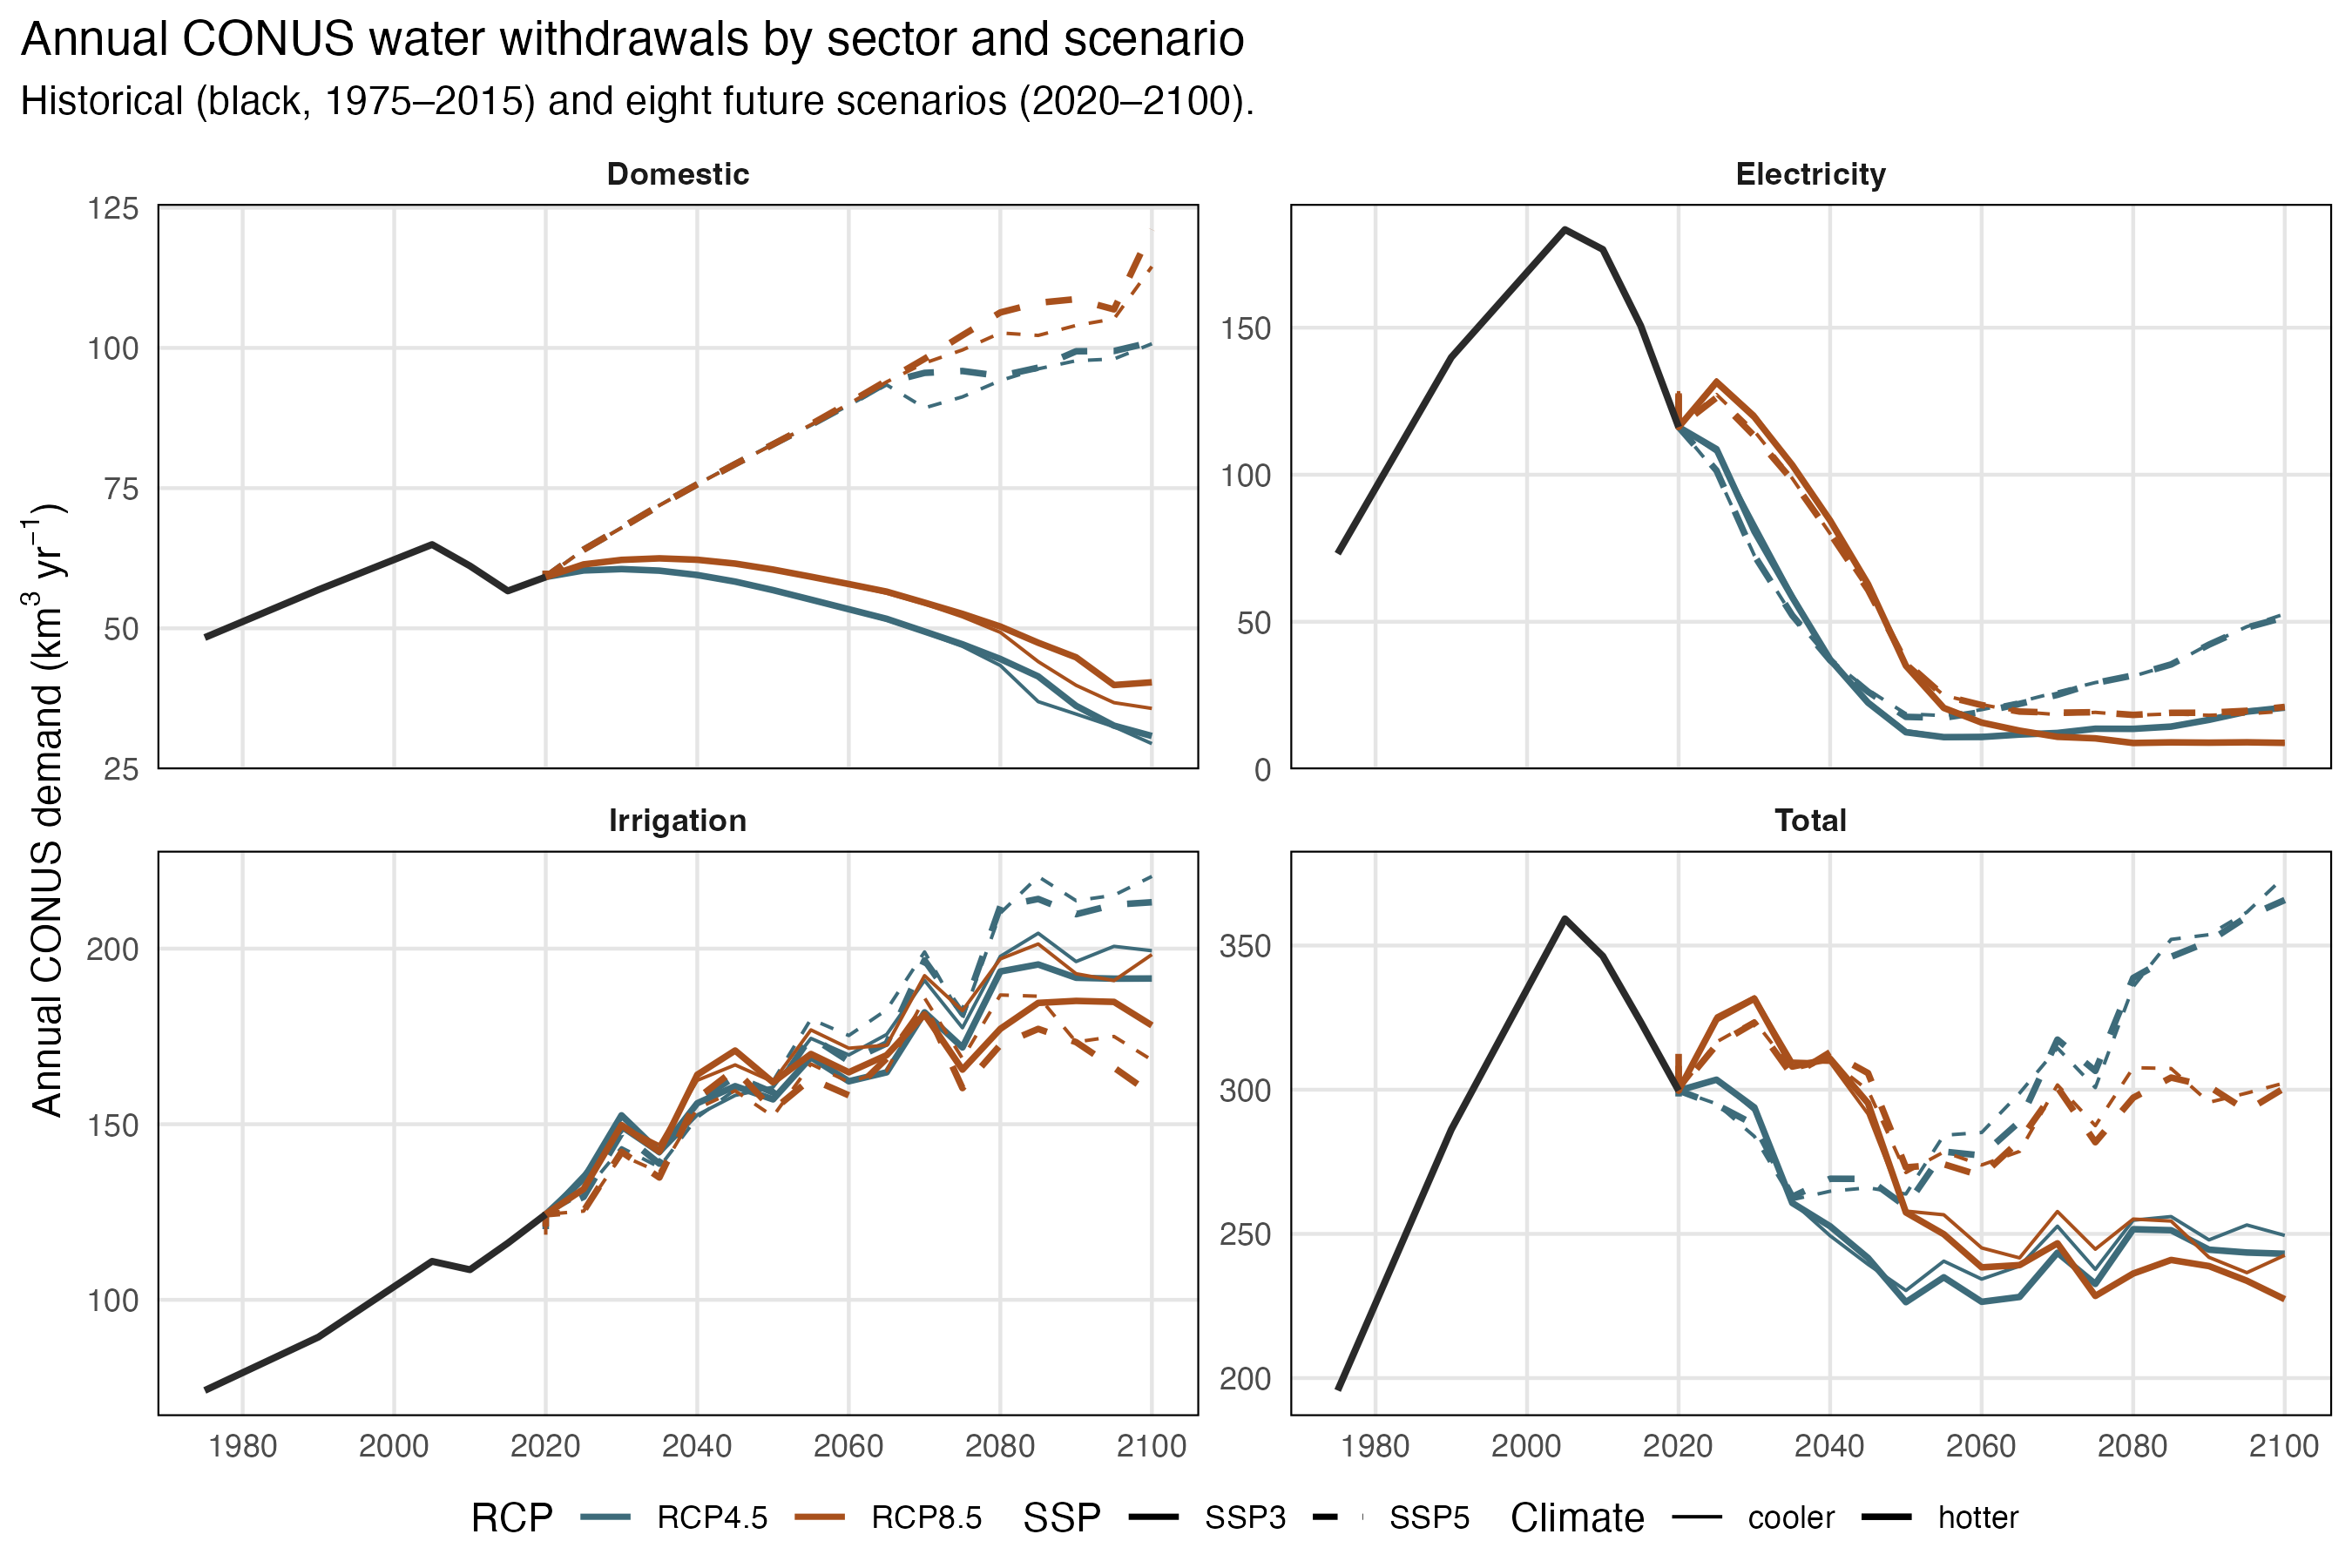
\includegraphics[width=\linewidth]{usage2-projections-annual-conus-timeseries.png}
\caption{Annual CONUS water withdrawals by sector and scenario. The historical simulation (black, 1975--2019) is connected to each of the eight future scenarios in 2020 for visual consistency; future scenarios vary by RCP (color), climate-model grouping (line width), and SSP (line style). Each panel uses an independent $y$-axis.}
\label{fig:scenarios}
\end{figure}

% \subsection*{HDD/CDD threshold sensitivity}

% The piecewise definition in Eq.~(\ref{eq:elec-cases}) describes four cases defined by specific HDD and CDD thresholds $H_{\mathrm{thr}}=650$ and $C_{\mathrm{thr}}=450$ from Huang et al.\cite{Huang2018}. We tested the sensitivity of the thresholds and the resulting monthly weights by perturbing the thresholds by $\pm 50\%$, holding the GCAM-USA shares $(p_{\mathrm{heat}}, p_{\mathrm{cool}}, p_{\mathrm{other}})$ fixed at $(0.20, 0.40, 0.40)$. Under the default thresholds, 32\% of CONUS cell-years fall in case~1 (both heating and cooling seasons present), 46\% in case~2 (heating only), 19\% in case~3 (cooling only), and 3\% in case~4 (uniform). Halving the thresholds to $(325, 225)$ moves the partition toward case~1 (49\%, 35\%, 16\%, 0\%); raising them by 50\% to $(975, 675)$ moves it toward case~2 (20\%, 54\%, 22\%, 5\%). The weights shifts the weights up by at most $\approx 1.8$ \% points and down by $\approx 1.1$~\% Figure~\ref{fig:eq5-sensitivity}. This indicated that the monthly Electricity weights are reasonably insensitive to the choice of HDD and CDD thresholds. 

%\begin{figure}[!ht]
%\centering
%
\includegraphics[width=.5\linewidth]{eq5-hdd-cdd-sensitivity.png}
%\caption{Sensitivity of Eq.~(\ref{eq:elec-cases}) to the HDD/CDD thresholds, computed over CONUS for the historical reference decade (2010--2019).}
%\label{fig:eq5-sensitivity}
%\end{figure}

\subsection*{Limitations}

Despite the advances presented above, several limitations should inform use of the dataset and motivate future work. Two limitations relate to the spatial stationarity of proxy fields. First, due to data limitations, the GLW~3 livestock distribution is held fixed at 2010 across all years and scenarios. This is reasonable as livestock represents a small share (only \textasciitilde2\%) of CONUS demand, but we recognize that within individual basins, particularly in states with rapidly shifting livestock composition, the static map may obscure local patterns worth resolving further in follow-up work upon new data availability. Secondly, population serves as the spatial proxy for manufacturing and mining, which captures the average pattern of labor-associated demand but misses site-specific industrial or mining facilities whose withdrawals can be large locally in a grid cell.

Three further limitations are methodological. The simplified GSI used for irrigation temporal downscaling (Eqs.~\ref{eq:gsi-components}--\ref{eq:gsi-monthly}) drops the vapour-pressure-deficit (VPD) component of the original Jolly et al.\cite{Jolly_2005} formulation; this simplification is consistent with Moore et al.\cite{Moore_2015} but may underweight drought months in humid climates where VPD is the binding constraint. Irrigation files are released both with and without conveyance losses applied (\texttt{\_with\_losses} suffix), and users coupling the dataset to hydrologic routing should select the appropriate variant for their application. Finally, the 5-year GCAM-USA time step is linearly interpolated to annual resolution, which suppresses interannual variability. This is most visible as smoother trend lines in irrigation and could be improved for using the dataset for replicating year-to-year demand variability beyond scenario-level and climatological-mean analyses.

% -----------------------------------------------------------------------------
\section*{Usage Notes}

This dataset functions as a high-resolution spatiotemporal representation of water demand and source dependence, enabling the coupling of sectoral water use with climate, hydrologic, energy, agricultural, and socioeconomic systems across historical and future scenarios through the end of 21$^{st}$ century. Several potential use cases have been curated as potential applications of this dataset, as summarized in Table \ref{tab:water_demand_roles}.

\begin{table}[!ht]
\centering
\small
\begin{tabular}{p{3.2cm} p{4.5cm} p{8.4cm}}
\hline
\textbf{Role} & \textbf{Description} & \textbf{Mechanism / Model Integration Use Cases} \\
\hline

Hydrologic and Earth System Forcing Variable &
Input to hydrologic, groundwater, and Earth system models as anthropogenic water demand across sectors &
Exogenous water use input as a demand component in water balance and scarcity calculations (e.g., demand/renewable supply), or as a model input in river routing, groundwater, or land-surface models such as MOSART-WM\cite{hess-17-4555-2013}, MODFLOW\cite{modflow6}, Superwell\cite{superwell}, ParFlow\cite{parflow}, VIC\cite{vic}, CLM\cite{clm5}, PCR-GLOBWB\cite{pcrglobwb}, and CWatM\cite{cwatm}. \\

Scenario and Coupling Driver &
Encodes future socioeconomic and climate pathways and connects water, energy, agriculture, land, and climate systems &
Future demand trajectories in integrated assessment models or regional impacts and adaptation studies as an information exchange mechanism linking hydrology, energy, and crop models, e.g., GCAM\cite{Calvin2019GCAM}, MESSAGEix\cite{messageix}, GLOBIOM\cite{globiom}, and CLIMADA\cite{climada}. \\

Decision-Support &
Supports planning, policy, resource management, and human decision making &
Input to optimization, reservoir operations, agent-based, and drought planning models for infrastructure investment analysis and water allocation planning, e.g., GEB\cite{geb}. \\

Feature Dataset &
Predictor variable for statistical and machine learning models &
Feature set for Random Forest, XGBoost, LSTM, GNN, and other predictive models for drought impacts, crop yields, groundwater depletion, water scarcity, and infrastructure risk. \\

\hline
\end{tabular}
\caption{Roles of the Tethys gridded water-demand dataset with representative model integrations and potential use cases for modeling communities and decision makers.}
\label{tab:water_demand_roles}
\end{table}

% other models that may use this: superwell, ECHO, GEB, CWatM, SimpleG etc - mostly hydroeco models. Can package into one of the above


More mechanically, we distribute the dataset as netCDF~4 files containing year and month dimensions. Each file contains either withdrawals or consumption in km$^3$~yr$^{-1}$. Users may convert from the native unit (km$^3$~yr$^{-1}$) to MGD by multiplying by $264{,}172.05124/365$, so $1\text{ km}^3\text{ yr}^{-1} \approx 723.76$~MGD.

The companion integration meta-repository (see "Code and external data availability") provides several tools and utilities for working with the dataset such as HUC-level aggregation utilities aggregations from the 1/8$^{\circ}$ grid to HUC2, HUC4, HUC6, HUC8, or HUC12 polygons; see the meta-repository README for details.

\section*{Improvements over previous data sets} \label{sec:improvements}

Compared with the prior Tethys global product\cite{Khan2023}, the dataset presented here advances the representation of U.S. water demand in six specific ways.

\paragraph{Resolution refinement.} Spatial resolution is refined from 1/2$^{\circ}$ to 1/8$^{\circ}$, a factor-of-4 improvement per dimension and a factor-of-16 improvement in areal resolution. Combined with finer proxy data (CERF plants at \textasciitilde1~km, Demeter LULC at 1/8$^{\circ}$, and SSP-compliant population at 1/8$^{\circ}$), the 1/8$^{\circ}$ resolution captures sub-state demand variation and is directly relevant to river routing, reservoir management, and local planning applications.

\paragraph{GCAM-USA integration.} The prior Tethys dataset used the global GCAM configuration, which disaggregated U.S.~demand from a single national total. This dataset uses GCAM-USA, which resolves U.S.~electricity generation, manufacturing, and municipal demand at the state level and crop irrigation demand at state/basin intersections. State-level inputs eliminate the artifact of national-average demand being pushed uniformly into states with very different sectoral mixes, and they allow the subsequent spatial downscaling to respect state-level regulatory boundaries — a distinction particularly important for regions such as the western U.S., where water law varies significantly across state lines.

\paragraph{CERF-based power-plant siting.} Prior electricity demand used population as the spatial proxy, which approximates the location of electricity load rather than the location of cooling water demand. This dataset uses explicit power-plant siting from the CERF model\cite{Vernon2021,Mongird2025CERF}, which places thermoelectric plants at $\approx$1-km resolution based on siting feasibility and then aggregates installed capacity to the 1/8$^{\circ}$ grid as the proxy. The result places thermoelectric demand at actual and projected generation sites rather than population centroids. For regions where thermoelectric demand dominates withdrawals, this correction substantially changes both the spatial pattern and the basin-scale water stress signal.

\paragraph{SSP-consistent population.} Prior work used a static base-year population map to distribute municipal, manufacturing, and mining demand across all years, including future projections. This dataset uses SSP3 and SSP5 gridded population projections from Jones and O'Neill\cite{Jones_2016}, linearly interpolated from their decadal native resolution to annual values. Scenario-consistent population is essential for the SSP-differentiated futures: SSP3 and SSP5 diverge markedly in U.S.~population growth, and that divergence propagates into the Domestic demand field in a way that a static map cannot represent.

\paragraph{GSI-based irrigation temporal downscaling.} Prior irrigation monthly weights used a simpler temperature-driven scheme. This dataset computes per-cell monthly weights (Eq.~\ref{eq:irr-weights}) from the monthly deficit and growing-season index, so the monthly distribution of irrigation demand responds to climate-consistent drought and growing-condition signals rather than to a static seasonal template. The monthly irrigation distribution thus varies from year to year and across scenarios, tracking interannual drought variability that a static template cannot reproduce.

\paragraph{Representation of groundwater/surface water split.} This is a novel contribution of this study with no prior work. We first apply GCAM's basin-level groundwater-to-surface split uniformly across all cells within a basin, then use Eq.~(\ref{eq:source-shares}) to combine GCAM-USA's temporal evolution of source shares with the finer-scale spatial distribution inferred from USGS groundwater and surface-water intake distributions at the HUC12 level, providing per-cell source attribution that is both temporally dynamic and spatially informed. This is essential for applications involving groundwater depletion, surface water availability, and conjunctive use modeling. 

Together, these six advances produce a much improved representation of CONUS water demands across sectors, scenarios, and scales. As discussed in Technical Validation, the annual totals are in close agreement with the latest USGS water-use data (January~2025) although the two datasets diverge in their spatial distribution at the basin scale. Users computing per-sector scarcity at individual basins should consult Table~\ref{tab:validation-metrics} and the HUC6 maps to assess the differences between the datasets before using the projected data.

% -----------------------------------------------------------------------------
\section*{Code and external data availability}

\begin{itemize}
    \item \textbf{Tethys downscaling package}\cite{niazi_2026_20552731}: \href{https://github.com/JGCRI/tethys}{github.com/JGCRI/tethys} 
    \item \textbf{Integration meta-repository}\cite{cambrackenIMMMSFATethys_integration_metarepoV1002026}: \href{https://github.com/IMMM-SFA/tethys_integration_metarepo}{github.com/IMMM-SFA/tethys\_integration\_metarepo} and the input dataset\cite{brackenDataTethys_integration_metarepo}. See the repository README for instructions on reproducing the dataset and figures in this paper.
    \item \textbf{TGW meteorology data}: The TGW climate forcing\cite{Jones2023TGW} that drives the Tethys runs is available as external data at \href{https://tgw-data.msdlive.org/}{tgw-data.msdlive.org}. 
    %\item \textbf{Demeter} (land-use downscaling, used to produce per-crop irrigated-area proxies): \url{https://github.com/IMMM-SFA/demeter}\cite{Vernon-2018}.
    %\item \textbf{CERF} (power-plant siting): \url{https://github.com/IMMM-SFA/cerf}\cite{Vernon2021}.
\end{itemize}


% -----------------------------------------------------------------------------
\section*{Acknowledgments}

This research was supported by the U.S.~Department of Energy, Office of Science, as part of research in Earth and Environmental System Modeling Program. We thank the TGW team for the downscaled climate product, the GCAM-USA team for the scenario simulations, and the USGS water-use program for the high-quality data used for evaluation in this paper.

\section*{Author contributions statement}

% TODO: coauthors to fill in per CRediT roles. Illustrative template:
C.B.~Coordinated the downscaling runs, conducted the HUC-scale comparison against USGS data, and drafted this version of the manuscript based on an earlier draft by I.T. 
H.N.~Developed and maintained the Tethys model, conducted the runs, and helped with the interpretation of GCAM-USA and Tethys outputs. 
T.T.~Extended the Tethys package to support GCAM-USA inputs, developed the first version of the Tethys metarepo, and carried out the initial scenario runs. 
I.T.~Wrote initial draft of this manuscript, contributed to the CERF--Tethys integration and power-plant proxy construction. 
K.T.~Developed the USGS-anchored groundwater-to-surface source-share attribution postprocessing framework for Tethys and conducted the associated runs and analyses. 
H.E.~Produced the TGW preprocessing pipeline for PET, HDD/CDD, and GSI. 
K.M.~Developed CERF--Tethys integration and power-plant proxy construction. 
N.V.~Contributed to scenario design and interpretation. 
N.S.~Scientific review, scenario design and interpretation. 
J.R.~Provided overall project guidance and scientific review. 

\section*{Competing interests}

The authors declare no competing interests.

\bibliography{bib/Tethys}

\end{document}
